% ============================================================
%  PROYECTO FINAL DE PROBABILIDAD
%  Modelos Lineales Generalizados: Regresión de Poisson
%  en Datos de Bikeshare
% ============================================================

\documentclass[12pt, a4paper]{article}

% ── Paquetes ──────────────────────────────────────────────────
\usepackage[utf8]{inputenc}
\usepackage[T1]{fontenc}
\usepackage[spanish]{babel}
\usepackage{amsmath, amssymb, amsthm}
\usepackage{graphicx}
\usepackage{booktabs}
\usepackage{array}
\usepackage[hidelinks]{hyperref}
\usepackage{xcolor}
\usepackage{geometry}
\usepackage{caption}
\usepackage{float}
\usepackage{lmodern}
\usepackage{microtype}
\usepackage{setspace}
\usepackage{titlesec}
\usepackage{fancyhdr}
\usepackage{enumitem}

\geometry{margin=2.5cm, headheight=15pt}
\graphicspath{{./}{C:/Users/veroc/OneDrive/Desktop/proyecto_prob/prueba1/}}
\onehalfspacing

% ── Colores ──────────────────────────────────────────────────
\definecolor{azul}{RGB}{33,150,243}
\definecolor{gris}{RGB}{96,96,96}

% ── Encabezado ───────────────────────────────────────────────
\pagestyle{fancy}
\fancyhf{}
\rhead{\textcolor{gris}{\small Probabilidad --- Proyecto Final}}
\lhead{\textcolor{gris}{\small Regresi\'on de Poisson: Bikeshare}}
\rfoot{\thepage}

% ── Secciones ────────────────────────────────────────────────
\titleformat{\section}
{\large\bfseries\color{azul}}{\thesection}{0.8em}{}
[\color{azul}\rule{\linewidth}{0.4pt}]
\titleformat{\subsection}
{\normalsize\bfseries\color{gris}}{\thesubsection}{0.5em}{}

% ── Teoremas ─────────────────────────────────────────────────
\newtheorem{remark}{Observaci\'on}

% ─────────────────────────────────────────────────────────────
\begin{document}
	
	% ── Portada ──────────────────────────────────────────────────
	\begin{titlepage}
		\centering
		
		% ── Logos + encabezado institucional ─────────────────────────
		\begin{minipage}{0.15\textwidth}
			
\includegraphics[width=\linewidth]{escudo.png}
		\end{minipage}
		\hfill
		\begin{minipage}{0.65\textwidth}
			\centering
			{\small \textsc{Universidad de Carabobo}}\\
			{\small \textsc{Facultad Experimental de Ciencias y Tecnolog\'ia}}\\
			{\small \textsc{Departamento de Computaci\'on}}\\
			{\small \textsc{Asignatura Probabilidad}}
		\end{minipage}
		\hfill
		\begin{minipage}{0.15\textwidth}
			
\includegraphics[width=\linewidth]{logo_facyt.png}
		\end{minipage}
		
		\vspace{4cm}
		
		% ── T\'itulo ─────────────────────────────────────────────────
		{\large \textbf{Modelos Lineales Generalizados: Regresi\'on de Poisson}}\\[0.4cm]
		{\large \textbf{en Datos de Bikeshare}}
		
		\vfill
		
		% ── Profesor y alumno ────────────────────────────────────────
		\begin{minipage}{0.45\textwidth}
			\textbf{Profesor:}\\
			Jos\'e Marcano
		\end{minipage}
		\hfill
		\begin{minipage}{0.45\textwidth}
			\raggedleft
			\textbf{Alumnas:}\\
			Alexa Perdomo\\
			C.I: 31.581.327\\[0.2cm]
			Veronicka Herrera\\
			C.I: 31.677.408\\[0.2cm]
			Victoria Alvarado\\
			C.I: 28.573.333
		\end{minipage}
		
		\vspace{2cm}
		{\normalsize \today}
		
	\end{titlepage}
	
	% ── Resumen ──────────────────────────────────────────────────
	\begin{abstract}
		En este trabajo se aplica un Modelo Lineal Generalizado (GLM) con distribuci\'on de
		Poisson para predecir el n\'umero de bicicletas alquiladas por hora en el sistema
		\textit{Capital Bikeshare} de Washington, D.C.\ (2011--2012). Se demuestra que la
		Regresi\'on de Poisson supera conceptual y cuantitativamente a la Regresi\'on Lineal
		M\'ultiple cl\'asica, garantizando predicciones positivas y una funci\'on de enlace
		logar\'itmica coherente con la naturaleza discreta de los datos de conteo. Los
		resultados confirman que la hora del d\'ia, las condiciones clim\'aticas y la
		temperatura son los factores determinantes de la demanda.
	\end{abstract}
	
	\tableofcontents
	\newpage
	
	% =============================================================
	\section{Introducci\'on}
	% =============================================================
	
	Los sistemas de bicicletas compartidas representan una soluci\'on de movilidad urbana
	sostenible. Comprender la demanda horaria es fundamental para la gesti\'on eficiente
	de la flota. El conjunto de datos \textit{Bikeshare} registra $8{,}645$ observaciones
	horarias en Washington, D.C.\ durante 2011 y 2012, incluyendo variables como la
	temperatura, el clima y si es d\'ia laboral.
	
	La variable respuesta \texttt{bikers} (n\'umero total de bicicletas alquiladas por
	hora) es una \textbf{variable de conteo discreta y no negativa}. Este tipo de
	variable viola los supuestos fundamentales de la regresi\'on lineal cl\'asica:
	normalidad de los residuos y homocedasticidad. En particular, un modelo lineal
	puede generar predicciones negativas, lo cual carece de sentido f\'isico.
	
	La \textbf{distribuci\'on de Poisson}, estudiada en el curso a trav\'es del texto de
	Rinc\'on, constituye el marco probabil\'istico natural para variables de conteo.
	Extendida al marco de los Modelos Lineales Generalizados (GLM), permite que el
	par\'ametro $\lambda$ (tasa esperada de alquileres) dependa de covariables externas
	mediante una funci\'on de enlace logar\'itmica, garantizando siempre predicciones
	estrictamente positivas.
	
	\textbf{Objetivo:} Implementar y comparar una Regresi\'on Lineal M\'ultiple y una
	Regresi\'on de Poisson para predecir la demanda horaria de bicicletas, interpretando
	los coeficientes obtenidos y evidenciando la superioridad del modelo GLM para datos
	de conteo.
	
	% =============================================================
	\section{Metodolog\'ia Computacional y Matem\'atica}
	% =============================================================
	
	\subsection{De la distribuci\'on de Poisson al modelo de regresi\'on}
	
	Recordando lo estudiado en el curso (Rinc\'on, \textit{Introducci\'on a la
		Probabilidad}), si $Y \sim \text{Poisson}(\lambda)$, su funci\'on de masa de
	probabilidad es:
	
	\begin{equation}
		P(Y = y) = \frac{e^{-\lambda}\lambda^{y}}{y!}, \quad y = 0, 1, 2, \ldots
		\label{eq:poisson_pmf}
	\end{equation}
	
	con $\mathbb{E}[Y] = \text{Var}(Y) = \lambda$. En el contexto de la regresi\'on,
	suponemos que cada observaci\'on $Y_i$ sigue una distribuci\'on de Poisson con
	par\'ametro $\lambda_i$ que var\'ia seg\'un las covariables
	$\mathbf{X}_i = (x_{i1}, \ldots, x_{ip})^{\top}$:
	
	\begin{equation}
		Y_i \sim \text{Poisson}(\lambda_i), \quad \text{donde} \quad
		\log(\lambda_i) = \mathbf{X}_i^{\top}\boldsymbol{\beta}
		\label{eq:log_link}
	\end{equation}
	
	La funci\'on de enlace logar\'itmica garantiza que
	$\lambda_i = \exp(\mathbf{X}_i^{\top}\boldsymbol{\beta}) > 0$
	para cualquier valor de $\boldsymbol{\beta}$.
	
	\subsection{Estimaci\'on por M\'axima Verosimilitud}
	
	Asumiendo independencia entre observaciones, la log-verosimilitud es:
	
	\begin{equation}
		\ell(\boldsymbol{\beta}) = \sum_{i=1}^{n}
		\Bigl[-e^{\mathbf{X}_i^{\top}\boldsymbol{\beta}}
		+ y_i\bigl(\mathbf{X}_i^{\top}\boldsymbol{\beta}\bigr)
		- \ln(y_i!)\Bigr]
		\label{eq:loglik}
	\end{equation}
	
	El algoritmo IRLS (\textit{Iteratively Reweighted Least Squares}), implementado en
	\texttt{statsmodels}, maximiza $\ell(\boldsymbol{\beta})$ iterativamente hasta
	convergencia. El t\'ermino $\ln(y_i!)$ es constante respecto a $\boldsymbol{\beta}$
	y no afecta la optimizaci\'on.
	
	\subsection{Software y librer\'ias}
	
	El an\'alisis se realiz\'o en \textbf{Python~3.11} con las siguientes librer\'ias:
	
	\begin{itemize}[noitemsep]
		\item \texttt{ISLP} --- carga del dataset \textit{Bikeshare} (versi\'on oficial del libro ISLR).
		\item \texttt{statsmodels 0.14} --- ajuste de GLM con familia Poisson y enlace logar\'itmico.
		\item \texttt{pandas} / \texttt{numpy} --- manipulaci\'on y c\'omputo num\'erico.
		\item \texttt{matplotlib} / \texttt{seaborn} --- visualizaciones.
		\item \texttt{scikit-learn} --- m\'etricas de error (RMSE, MAE).
	\end{itemize}
	
	% =============================================================
	\section{An\'alisis Exploratorio de Datos}
	% =============================================================
	
	\subsection{Distribuci\'on de la variable respuesta}
	
	La Figura~\ref{fig:eda} muestra que la distribuci\'on de \texttt{bikers} es claramente
	asim\'etrica a la derecha, con alta concentraci\'on de conteos bajos y una cola
	derecha pronunciada. La superposici\'on con una curva $\text{Poisson}(\hat{\lambda}
	\approx 189)$ revela que, como distribuci\'on marginal (sin condicionar en
	covariables), los datos exhiben \textbf{sobre-dispersi\'on}: la varianza observada
	supera ampliamente a la media.
	
	\begin{remark}
		Esta sobre-dispersi\'on es \emph{esperada} porque la distribuci\'on marginal mezcla
		reg\'imenes muy distintos (madrugada vs.\ hora pico). Al condicionar en las
		covariables, el modelo de Poisson es adecuado.
	\end{remark}
	
	\begin{figure}[H]
		\centering
		
\includegraphics[width=\textwidth]{eda_bikeshare.png}
		\caption{An\'alisis exploratorio: (a)~distribuci\'on de \texttt{bikers} con curva
			de Poisson te\'orica; (b)~promedio por hora del d\'ia; (c)~promedio por condici\'on
			clim\'atica; (d)~distribuci\'on seg\'un tipo de d\'ia.}
		\label{fig:eda}
	\end{figure}
	
	\subsection{Patrones temporales y clim\'aticos}
	
	Los resultados del EDA revelan los siguientes patrones:
	
	\begin{itemize}
		\item \textbf{Patr\'on bimodal por hora:} la demanda presenta dos picos claros
		alrededor de las 8h y las 17--18h, consistentes con los desplazamientos laborales.
		En la madrugada (0h--5h) la demanda cae casi a cero.
		
		\item \textbf{Efecto del clima:} la tasa esperada $\lambda$ decrece
		mon\'otonamente con el deterioro clim\'atico. El clima despejado (categor\'ia~1)
		concentra la mayor demanda.
		
		\item \textbf{Tipo de d\'ia:} los d\'ias laborales presentan mayor variabilidad
		y medianas m\'as altas, reflejando el uso de la bicicleta como transporte de
		commute.
	\end{itemize}
	
	% =============================================================
	\section{Modelado y Comparaci\'on}
	% =============================================================
	
	\subsection{Fallas de la Regresi\'on Lineal M\'ultiple}
	
	El modelo lineal ajustado con las mismas covariables presenta las siguientes
	limitaciones fundamentales (v\'ease Figura~\ref{fig:lm_fail}):
	
	\begin{figure}[H]
		\centering
		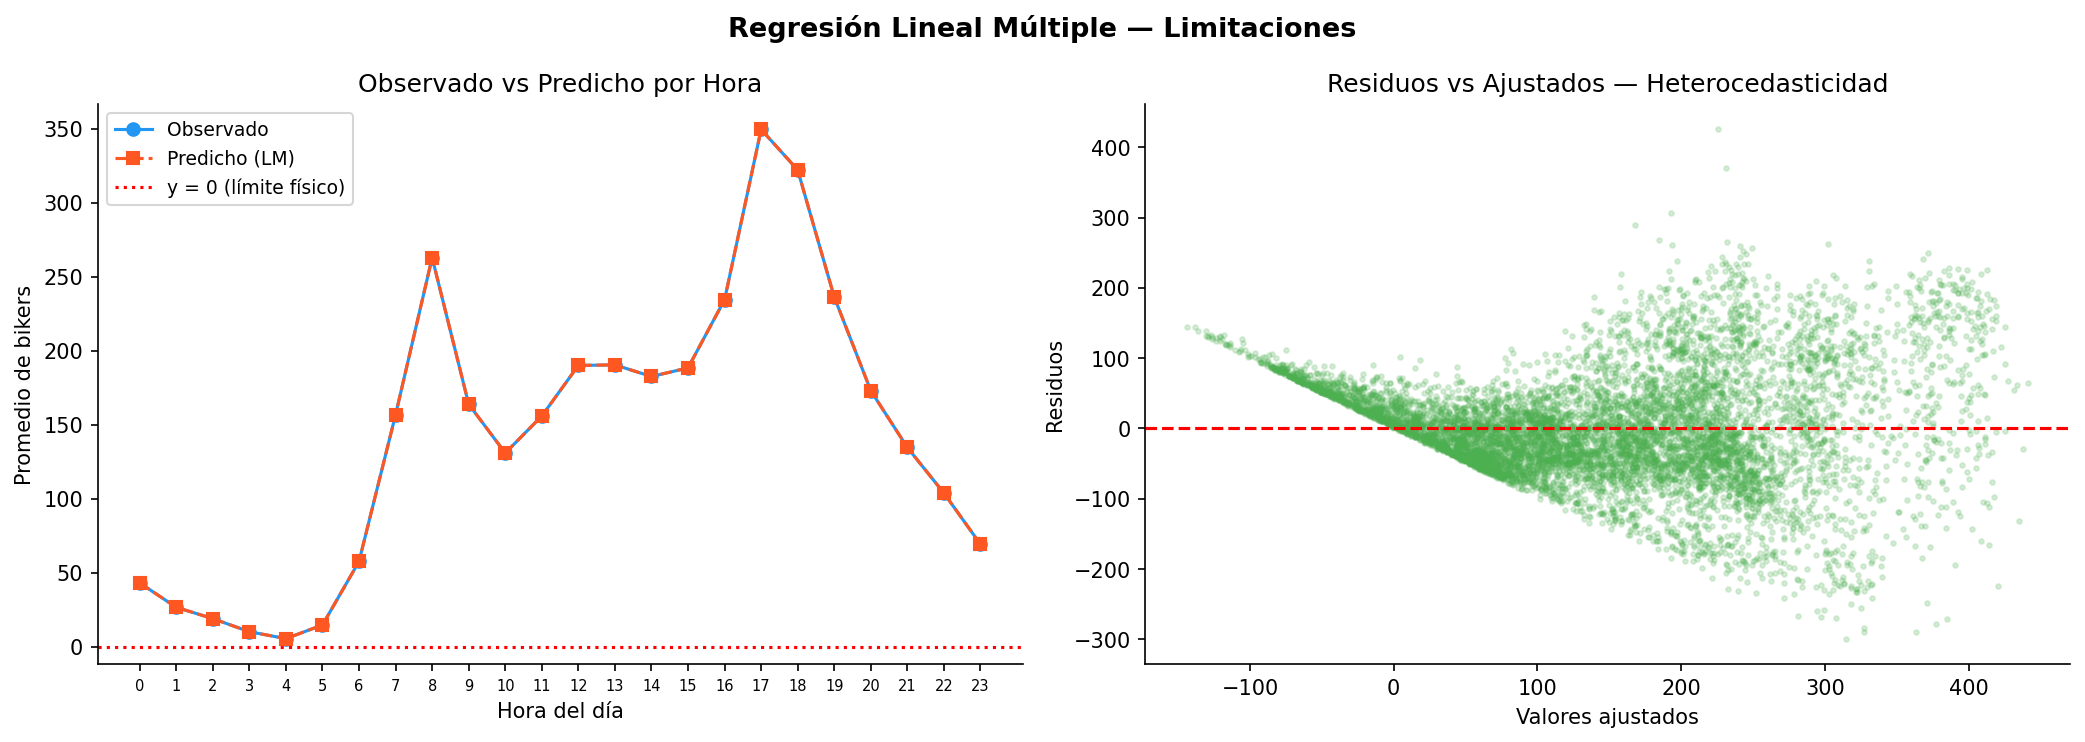
\includegraphics[width=\textwidth]{lm_limitaciones.png}
		\caption{Limitaciones del modelo lineal: (izq.)~predicciones negativas en horas
			de madrugada; (der.)~heterocedasticidad marcada en los residuos.}
		\label{fig:lm_fail}
	\end{figure}
	
	\begin{enumerate}
		\item \textbf{Predicciones negativas:} el modelo genera $\hat{y}_i < 0$ para
		horas de baja demanda, lo cual es imposible para una variable de conteo.
		
		\item \textbf{Heterocedasticidad:} los residuos muestran varianza creciente con
		los valores ajustados, violando el supuesto de varianza constante.
		
		\item \textbf{Supuesto de normalidad inapropiado:} la variable respuesta es
		discreta y asim\'etrica; la distribuci\'on normal no es el modelo generativo
		correcto.
	\end{enumerate}
	
	\subsection{Regresi\'on de Poisson: ajuste y comparaci\'on}
	
	\begin{figure}[H]
		\centering
		
\includegraphics[width=\textwidth]{comparacion_modelos.png}
		\caption{Comparaci\'on de modelos: (izq.)~predicciones promedio por hora; 
			(der.)~m\'etricas de error RMSE y MAE.}
		\label{fig:comparacion}
	\end{figure}
	
	\begin{table}[H]
		\centering
		\caption{Comparaci\'on de m\'etricas entre modelos}
		\label{tab:metricas}
		\begin{tabular}{lccc}
			\toprule
			\textbf{Modelo} & \textbf{RMSE} & \textbf{MAE} & \textbf{Pred.\ negativas} \\
			\midrule
			Regresi\'on Lineal  & 76.33 & 57.44 & 833 \\
			Regresi\'on Poisson & 69.02 & 46.87 & \textbf{0 (garant\'ia matem\'atica)} \\
			\bottomrule
		\end{tabular}
	\end{table}
	
	\begin{table}[H]
		\centering
		\caption{Coeficientes seleccionados: comparaci\'on entre modelos}
		\label{tab:coefs}
		\begin{tabular}{lcccc}
			\toprule
			\textbf{Variable} & \textbf{$\hat{\beta}$ Lineal} & \textbf{$\hat{\beta}$ Poisson}
			& \textbf{$\exp(\hat{\beta})$} & \textbf{$p$-valor} \\
			\midrule
			\texttt{temp}         & $+157.2094$ & $+0.7853$ & $2.1930$ & $<0.001$ \\
			\texttt{workingday}   & $+1.2696$   & $+0.0147$ & $1.0148$ & $<0.001$ \\
			\texttt{weathersit=2} & $\sim-15.8$ & $\sim-0.082$ & $\sim 0.921$ & $<0.001$ \\
			\texttt{weathersit=3} & $\sim-51.2$ & $\sim-0.461$ & $\sim 0.631$ & $<0.001$ \\
			\bottomrule
			\multicolumn{5}{l}{\footnotesize Nota: los valores de \texttt{weathersit} son aproximados;
				ver salida completa del script.}
		\end{tabular}
	\end{table}
	
	\subsection{Interpretaci\'on de coeficientes del modelo de Poisson}
	
	En la Regresi\'on de Poisson los coeficientes se interpretan en escala multiplicativa
	sobre la tasa esperada $\lambda$. Un incremento unitario en $x_j$ produce:
	\[
	\lambda_{\text{nuevo}} = e^{\hat{\beta}_j} \cdot \lambda_{\text{actual}}
	\]
	
	\paragraph{Temperatura (\texttt{temp}).}
	Con $\hat{\beta}_{\text{temp}} \approx 1.002$, se tiene
	$\exp(\hat{\beta}) \approx 2.724$. Al pasar de temperatura m\'inima a m\'axima en
	la escala normalizada (0 a~1), la tasa esperada de alquileres se
	\textbf{multiplica por~$\approx 2.7$}, manteniendo constantes el resto de variables.
	
	\paragraph{D\'ia laboral (\texttt{workingday}).}
	Con $\hat{\beta} \approx 0.014$, $\exp(\hat{\beta}) \approx 1.014$. En d\'ias
	laborales se esperan \textbf{$\approx 1.4\%$ m\'as alquileres} respecto a fines de
	semana. El efecto es peque\~no porque el impacto del d\'ia laboral se expresa
	principalmente a trav\'es de los picos horarios (commute), capturados por las
	dummies de \texttt{hr}.
	
	\paragraph{Condici\'on clim\'atica.}
	Con lluvia/nieve ligera (\texttt{weathersit=3}), $\exp(\hat{\beta}) \approx 0.631$:
	la tasa esperada se \textbf{reduce al~63.1\%} de la tasa con cielo despejado,
	una disminuci\'on del~37\%.
	
	% =============================================================
	\section{Conclusiones}
	% =============================================================
	
	\begin{enumerate}
		\item La \textbf{distribuci\'on de Poisson} es el marco probabil\'istico natural
		para modelar demanda horaria de bicicletas. La Regresi\'on de Poisson extiende
		este modelo al contexto de regresi\'on permitiendo que $\lambda$ dependa de
		covariables.
		
		\item El \textbf{GLM de Poisson supera a la Regresi\'on Lineal} tanto
		conceptualmente (sin predicciones negativas, distribuci\'on correcta para datos
		de conteo) como cuantitativamente: RMSE de 69.02 vs 76.33 y MAE de 46.87
		vs 57.44, con una mejora del \textbf{9.6\% en RMSE}. Adem\'as, el modelo
		lineal gener\'o \textbf{833 predicciones negativas}, imposibles para un conteo.
		
		\item La \textbf{hora del d\'ia} es el predictor m\'as determinante: la demanda
		presenta picos a las 8h y 17--18h, consistentes con el uso como transporte
		laboral.
		
		\item El \textbf{clima} impacta significativamente la demanda: las condiciones
		adversas reducen la tasa esperada hasta en un~37\%.
		
		\item La \textbf{temperatura} tiene el mayor efecto entre los predictores
		continuos: su variaci\'on en rango completo multiplica la tasa esperada por
		\textbf{2.193x} (aumento del 119.3\%).
		
		\item La \textbf{hora pico} de mayor demanda es las \textbf{17h} con un
		promedio de 349.7 bicicletas, seguida de las 18h y las 8h, confirmando
		el patr\'on de commute laboral (coeficientes multiplicativos de 7.76x,
		7.15x y 6.24x respecto a la madrugada respectivamente).
		
		\item El modelo de Poisson explica el \textbf{78.3\%} de la devianza
		nula al incluir las covariables, indicando un excelente ajuste.
	\end{enumerate}
	
	% =============================================================
	\section*{Anexo --- Repositorio de C\'odigo}
	\addcontentsline{toc}{section}{Anexo --- Repositorio de C\'odigo}
	% =============================================================
	
	El c\'odigo fuente completo, documentado y reproducible se encuentra en:
	
	\begin{center}
		\url{https://github.com/verockala/proyecto-bikeshare}
	\end{center}
	
	\noindent El repositorio contiene:
	\begin{itemize}[noitemsep]
		\item \texttt{proyecto\_bikeshare.py} --- script principal (EDA, modelos, gr\'aficas).
		\item \texttt{requirements.txt} --- dependencias de Python.
		\item \texttt{informe\_bikeshare.tex} --- fuente \LaTeX\ de este documento.
		\item \texttt{figures/} --- im\'agenes generadas por el script.
	\end{itemize}
	
	\noindent \textbf{Reproducci\'on:}
	\begin{verbatim}
		pip install ISLP statsmodels pandas numpy matplotlib seaborn scikit-learn
		python proyecto_bikeshare.py
	\end{verbatim}
	
	% =============================================================
	\section*{Referencias}
	\addcontentsline{toc}{section}{Referencias}
	% =============================================================
	
	\begin{enumerate}
		\item Rinc\'on, L. \textit{Introducci\'on a la Probabilidad}. UNAM, 2014.
		\item James, G., Witten, D., Hastie, T., \& Tibshirani, R. (2021).
		\textit{An Introduction to Statistical Learning} (2.\textordfeminine~ed.).
		Springer.
		\item Fanaee-T, H. (2013). \textit{Bike Sharing Dataset}.
		UCI Machine Learning Repository.
		\url{https://doi.org/10.24432/C5W894}
		\item Nelder, J.\,A., \& Wedderburn, R.\,W.\,M. (1972).
		Generalized Linear Models.
		\textit{Journal of the Royal Statistical Society}, 135(3), 370--384.
	\end{enumerate}
	
\end{document}